% !TeX program = xelatex
\documentclass[UTF8,11pt,a4paper,fontset=fandol]{ctexart}
\usepackage[left=23mm,right=23mm,top=20mm,bottom=22mm]{geometry}
\usepackage{xcolor,booktabs,tabularx,array,listings,textcomp,fancyhdr,enumitem,graphicx,url}
\definecolor{ink}{HTML}{173746}
\definecolor{accent}{HTML}{006C70}
\definecolor{muted}{HTML}{4B626D}
\definecolor{paper}{HTML}{F1F5F6}
\setlength{\parindent}{0pt}
\setlength{\parskip}{4pt}
\setlength{\emergencystretch}{3em}
\setlist{leftmargin=*,topsep=3pt,itemsep=1.5pt,parsep=1pt}
\ctexset{section={format=\Large\bfseries\color{ink},numbering=false,
  beforeskip=0pt,afterskip=8pt},
  subsection={format=\large\bfseries\color{accent},numbering=false,
  beforeskip=8pt,afterskip=3pt}}
\pagestyle{fancy}\fancyhf{}
\fancyhead[L]{\small\color{muted}本地文件批处理工具}
\fancyhead[R]{\small\color{muted}独立复现实验手册}
\fancyfoot[R]{\small\color{muted}\thepage}
\setlength{\headheight}{15pt}
\renewcommand{\headrulewidth}{0.3pt}
\lstset{basicstyle=\ttfamily\small,columns=fullflexible,keepspaces=true,
  showstringspaces=false,upquote=true,breaklines=true,backgroundcolor=\color{paper},
  frame=single,rulecolor=\color{paper},framesep=4pt,xleftmargin=5pt,xrightmargin=5pt,
  aboveskip=6pt,belowskip=6pt}
\newcommand{\file}[1]{\texttt{\detokenize{#1}}}
\newcommand{\partlabel}[1]{{\small\bfseries\color{accent}#1}\par}
\newcolumntype{Y}{>{\raggedright\arraybackslash}X}
\renewcommand{\arraystretch}{1.22}
\begin{document}

\partlabel{使用与交付}
{\Huge\bfseries\color{ink}归档台 · 文件批处理工作站\par}
\vspace{4pt}
双击“归档台.exe”进入桌面窗口，按任务选择规则。前五页从零实现“一键归档”，第 6 页起介绍各工具、表格计算和规则重放。每条订单可追溯到原文件和行号。

\subsection{先运行一批}
把 \file{batch_tool.py} 和 \file{requirements.txt} 放在同一个文件夹，在该位置打开 PowerShell。使用 Python 3.9 或更高版本。以下命令直接使用虚拟环境里的解释器。将待处理文件放入 \file{inbox}，或先按下一页生成样例。
\begin{lstlisting}
python -m venv .venv
.\.venv\Scripts\python.exe -m pip install -r requirements.txt
.\.venv\Scripts\python.exe batch_tool.py inbox out --format jpeg --sharpen
\end{lstlisting}
安装依赖后即可断网运行。\file{--format png} 保留透明通道；默认生成 JPEG，透明处铺白底。\file{--sharpen} 开启轻度锐化，省略时只做方向校正和格式转换。

\subsection{去哪里看结果}
终端会打印本次批次目录。每次运行都会生成一个新批次，源文件保留在原位置。

\begin{tabularx}{\linewidth}{@{}lY@{}}\toprule
\textbf{批次内的文件} & \textbf{内容与用途}\\\midrule
合并数据.xlsx & 所有 CSV 和 XLSX 工作表按列名对齐。前三列记录来源文件、工作表和原行号。\\
图片/、文档/ & 输出名为“扫描序号\_原名.后缀”。同名文件分别保存，清单给出原路径与新路径。\\
处理清单.json & 每个文件的结果、失败或跳过原因，以及文件数和合并行数。文本编码为 UTF-8。\\
整理结果.zip & 含上述工作簿、清单和已生成的图片及文档副本，可以直接解压检查。\\\bottomrule
\end{tabularx}

\subsection{输入约定}
CSV 使用逗号分隔，先尝试 UTF-8（含 BOM），解码失败后尝试 GB18030。XLSX 读取全部工作表。各表第一条非空记录是表头，一张表表达一类记录；建议同一批放业务含义一致的数据。列名统一后才能对齐，例如“货号”和“SKU”会保留为两列。

图片支持 JPEG、PNG、BMP、WebP、TIFF 和 GIF 的单帧文件。文档按扩展名复制，支持 DOC、DOCX、PDF、PPT、PPTX、TXT、MD、RTF。其他后缀和 Office 临时文件在清单中标为跳过。

\newpage
\partlabel{动手样例}
\section{先造一批能算出答案的输入}
把下方代码存为 \file{make_sample.py}，与主脚本放在一起。在该目录运行以下命令。样例需要新建 \file{inbox}；也可以按同样的行列和文件名手工制作。
\begin{lstlisting}
.\.venv\Scripts\python.exe make_sample.py
\end{lstlisting}

\begin{lstlisting}[language=Python]
from pathlib import Path
from openpyxl import Workbook
from PIL import Image

root = Path("inbox")
root.mkdir()
east, west = root / "east", root / "west"
east.mkdir()
west.mkdir()
(east / "orders.csv").write_text(
    "sku,qty\n0012,2\n\nNA,3\n", encoding="utf-8-sig")

book = Workbook()
orders = book.active
orders.title = "orders"
orders.append(["qty", "sku", "note"])
orders.append([4, "0012", "rush"])
returns = book.create_sheet("returns")
returns.append(["sku", "note"])
returns.append(["0009", "return"])
book.save(west / "orders.xlsx")

photo = Image.new("RGBA", (40, 30), (0, 0, 0, 0))
photo.paste((20, 100, 180, 255), (10, 8, 30, 22))
photo.save(east / "photo.png")
photo.save(west / "photo.png")
(west / "readme.txt").write_text("delivery note\n", encoding="utf-8")
(root / "unknown.bin").write_bytes(b"sample")
\end{lstlisting}

\subsection{运行前写下预期值}
输入共有六个文件。两张同名图都应出现；来自不同目录的文件由相对路径区分。CSV 有一条空记录，两个 Excel 工作表各有一条数据。最终应为\textbf{成功 5 个、失败 0 个、跳过 1 个、合并 4 行}。CSV 第一列中的 \file{0012} 和 \file{NA} 均应保留原文。带着这些预期值再运行首页的批处理命令。

\newpage
\partlabel{从空文件实现 · 数据}
\section{先做出一张能追溯的合并表}
\subsection{第一步：能解释每个输入从哪里来}
新建自己的 \file{batch_tool.py}。先只接收输入、输出两个目录，用 \file{argparse} 打印参数，然后用 \file{os.walk} 枚举输入。对每层目录和文件名排序，打印 \file{path.relative_to(root)}。用上一页的样本对照一次，两个 \file{photo.png} 应有不同的相对路径。把输出放在输入的子目录再试一次，递归前从 \file{dirs[:]} 删除输出目录。正式脚本的 \file{input_files} 实现了这一步。

\subsection{第二步：一次只读一张表}
先用 \file{csv.reader} 读取 CSV 并打印每条记录的编号。用 \file{enumerate(rows, 1)} 在清除空行之前编号。在样本里 \file{NA} 的编号应是 4。带引号的多行 CSV 字段仍占一条记录；Excel 的编号就是工作表行号。

接着用 \file{load_workbook(..., read_only=True, data_only=False)} 打开 XLSX，把每个工作表的 \file{sheet.values} 交给同一个函数。第一条非空记录给出列名，数据行去除文本首尾空白，短行尾部补空值。重复列名、表头中间缺名或数据宽过表头时，报出工作表与行号。一个工作簿的所有工作表读取成功后再收下整本数据，避免坏表造成半本入账。

\subsection{第三步：手算一次“按名对齐”}
东区表头为 \file{sku,qty}，西区为 \file{qty,sku,note}。先按首次遇到的次序收集列名，得到 \file{sku,qty,note}。打开 Python 解释器，做下面的最小实验。
\begin{lstlisting}[language=Python]
import pandas as pd
west = pd.DataFrame([[4, "0012", "rush"]],
                    columns=["qty", "sku", "note"], dtype=object)
aligned = west.reindex(columns=["sku", "qty", "note"])
assert aligned.iloc[0].tolist() == ["0012", 4, "rush"]
\end{lstlisting}
把三列来源信息放在业务列之前。用同一组列名依次对齐每个数据块，逐行交给 openpyxl，缺失值写成空单元格。遇到字符串显式设置单元格类型为 \file{s}，这样以等号开头的文本和 Excel 公式原文都按文本保存。CSV 的字段保留文本类型，Excel 数值保留数值类型。样式显示为 0012、底层值为 12 的 Excel 数值会输出 12；需要保留前导零的业务编号应在输入中存为文本。

\subsection{给自己设一个检查点}
只完成表格部分时先打开工作簿，确认 \file{west/orders.xlsx} 的订单行中，\file{sku} 是 \file{0012}，\file{qty} 是数值 4，\file{note} 是 \file{rush}。若 4 落到 \file{sku} 列，回到对齐步骤打印两张表的列名。重复订单行会保留，便于核对原始记录。

\newpage
\partlabel{从空文件实现 · 文件与图片}
\section{给每个文件一条能核对的去向}
\subsection{第四步：先转换一张透明 PNG}
在样例上运行下面的片段，观察透明角落转成 JPEG 后的颜色。JPEG 无透明通道，需要用原图的 alpha 作为蒙版，把可见内容贴到白色画布上。手机照片先按 EXIF 方向旋转，再执行后续处理。
\begin{lstlisting}[language=Python]
from PIL import Image, ImageOps, ImageFilter
with Image.open("inbox/east/photo.png") as src:
    rgba = ImageOps.exif_transpose(src).convert("RGBA")
    alpha = rgba.getchannel("A")
    rgb = rgba.convert("RGB")
    rgb = rgb.filter(ImageFilter.UnsharpMask(
        radius=1.2, percent=110, threshold=3))
    canvas = Image.new("RGB", rgb.size, "white")
    canvas.paste(rgb, mask=alpha)
    canvas.save("preview.jpg", quality=90, subsampling=0)
\end{lstlisting}
在正式脚本里把滤镜放进 \file{--sharpen} 分支。半径控制参与计算的邻域，百分比控制边缘增强幅度，阈值让较小的亮度变化绕过滤镜。PNG 输出时把原 alpha 装回 RGB 图。用同一张图分别开启、关闭锐化，在原尺寸下检查文字边缘；过强会出现光晕，严重失焦也无法靠锐化还原。多帧图片记录失败，避免只输出第一帧。

\subsection{第五步：再做批量命名和清单}
对已排序的扫描结果编号，例如 \file{0003_photo.jpg}。序号来自全部输入文件，跳过项也占一号。用 \file{shutil.copy2} 复制文档。每处理一个文件，就保留它的相对路径、状态、输出位置或原因。试着把普通文本改名为 \file{broken.jpg} 加入输入：图片解码应失败，下一份文件应继续处理，结果中应有一条带输入名的错误记录。

\subsection{第六步：最后生成压缩包}
先在输出根目录下新建临时目录，把工作簿、图片、文档和清单写齐。创建 ZIP 前列出要打包的文件；调用 \file{archive.write(path, arcname)} 时，用相对批次目录的路径作为包内名。用 \file{ZipFile.testzip()} 检查，返回 \file{None} 表示各成员 CRC 检查通过。收尾时把临时成品目录改为新的批次名。

忘记接口参数时，在已安装依赖的 Python 解释器里输入 \file{help(zipfile.ZipFile.write)} 或 \file{help(Image.Image.paste)}，先导入对应模块。练习时每次只实现上面的一步，先预测样例输出，再用打印、断点或断言核对。合上参考脚本后，用相同样例测试自己写的版本，并记录第一处结果差异。

\newpage
\partlabel{验收与排错}
\section{用结果判断哪一步写对了}
\subsection{核对合并数据}
用第二页的原始样例运行后，三个来源列应分别为“\_\_来源文件”“\_\_工作表”“\_\_原行号”。下表用短列名展示预期值，横线表示空单元格。

\begin{tabularx}{\linewidth}{@{}Ylllll@{}}\toprule
\textbf{来源文件} & \textbf{表} & \textbf{原行号} & \textbf{sku} & \textbf{qty} & \textbf{note}\\\midrule
\file{east/orders.csv}  & — & 2 & 0012 & 2 & —\\
\file{east/orders.csv}  & — & 4 & NA   & 3 & —\\
\file{west/orders.xlsx} & orders & 2 & 0012 & 4 & rush\\
\file{west/orders.xlsx} & returns & 2 & 0009 & — & return\\\bottomrule
\end{tabularx}

\subsection{核对图片、文档与归档}
\begin{enumerate}
\item 打开“图片”目录。两个 JPEG 都应为 $40\times30$ 像素，左上角为白色。改用 \file{--format png} 再运行，在新批次检查相同角落的 alpha 为 0。旧批次仍应可打开。
\item 打开“处理清单.json”。找到 \file{west/readme.txt} 的输出路径，用 PowerShell 的 \file{Get-FileHash} 分别计算原文档与副本的 SHA256，两值应相等。找到 \file{unknown.bin}，状态应为 \file{skipped}。
\item 解压 ZIP。基础样例中应有\textbf{五个文件}：一份工作簿、一份清单、两张图片和一份文档。对照清单检查归档路径与磁盘上的相对路径一致。
\end{enumerate}

\subsection{故意改变一个条件，再看反馈}
\begin{tabularx}{\linewidth}{@{}p{.37\linewidth}Y@{}}\toprule
\textbf{操作} & \textbf{预期与定位}\\\midrule
加入损坏的 JPG 后重跑 & 退出码 1；在清单中按 \file{status=error} 找到该文件。其他正常文件仍有产物。\\
将 CSV 表头改成 \file{sku,sku} & 该 CSV 失败，原因中有行号；原样例中的 Excel 仍贡献两条数据。\\
输入指向不存在的目录 & 退出码 2；终端给出失败原因。先检查路径和引号。\\
把输出改为 \file{inbox/out}，连续运行两次 & 两次得到不同批次；原始样例每次都是 4 行，历史输出不会被再次读入。\\\bottomrule
\end{tabularx}

\subsection{交付时能说明的边界}
PowerShell 中用 \file{$LASTEXITCODE} 查看脚本退出码。只有跳过项时仍可返回 0。表格数据块保存在内存中，最终写入一张工作表；超过 Excel 的 1,048,576 行（含表头）或 16,384 列时需分批运行。处理清单可把成功、跳过和失败区分开来，便于决定本批次是否交付。
\newpage
\partlabel{桌面工作台}
\section{从文件选择到结果预览}
双击“归档台.exe”或“启动工作台.cmd”。顶部标签选择任务，左栏设置目录、指定文件和规则，右栏可筛选状态、核对样本、导出清单。“预览结果”只计算，“执行处理”重新读取当前输入并生成新批次。输出目录留空时使用输入目录内的“整理结果”。
\begin{center}
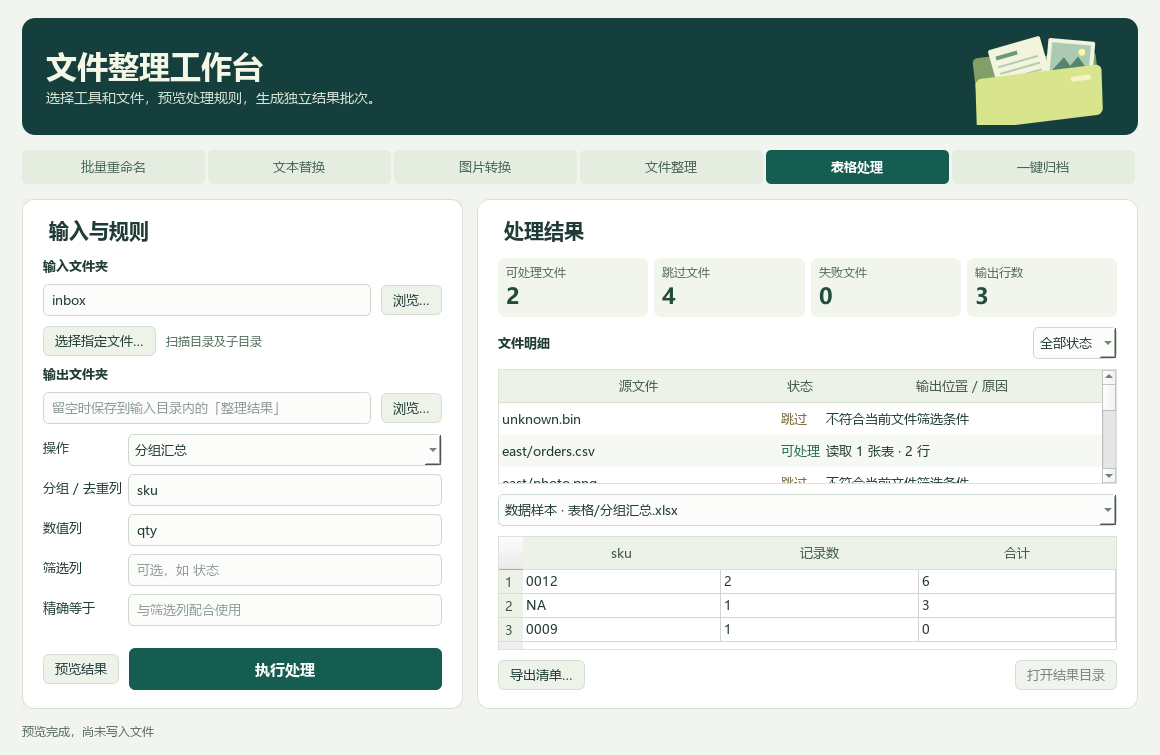
\includegraphics[width=\linewidth,height=.39\textheight,keepaspectratio]{docs/workbench.png}
\end{center}
上图是第 2 页样例的真实预览：以 \file{sku} 分组，对 \file{qty} 求和。右下角可查看实际数据，批次尚未写入磁盘。

\begin{tabularx}{\linewidth}{@{}lY@{}}\toprule
\textbf{工具} & \textbf{操作与结果}\\\midrule
批量重命名 & 模板序号、查找替换、前后缀、后缀筛选。默认输出副本；勾选原位改名可修改原件并在本次会话撤销最近一次改名。\\
文本替换 & 普通文本、正则表达式、捕获组引用、大小写和编码选项。列出匹配次数与首个匹配示例。\\
图片转换 & 输出 JPEG、PNG、WebP、BMP 或 TIFF。JPEG/WebP 可调编码质量，支持方向校正与轻度锐化。\\
文件整理 & 按类型或修改月份分类。内容查重生成 CSV，列出同组的全部相对路径。\\
表格处理 & 合并、筛选、列选择、跨表去重、分组汇总、按值拆分，以及 CSV/XLSX 互转。\\
一键归档 & 执行前五页的组合流程，一次生成工作簿、图片、文档副本与 ZIP。\\\bottomrule
\end{tabularx}
\newpage
\partlabel{表格实操}
\section{用四条订单验证六种操作}
按第 2 页建样例，选“表格处理”，输入目录填 \file{inbox}。两个表格文件参与处理，其他四个输入在清单中显示为跳过。每次只改变一个条件，再对照预期。

\begin{tabularx}{\linewidth}{@{}p{.22\linewidth}YY@{}}\toprule
\textbf{目标} & \textbf{操作} & \textbf{验收标准}\\\midrule
筛选及选择列 & 按列合并；筛选列 \file{note} 等于 \file{rush}；保留列 \file{qty,sku} & 输出一行。三列来源信息后依次是数值 4 和文本 0012。\\
跨文件去重 & 按键去重；键为 \file{sku}；清空筛选 & 保留三行，0012 只出现一次，来自首次读取的东区文件。\\
分组汇总 & 分组列 \file{sku}；数值列 \file{qty} & 0012 有两条，合计 6；NA 合计 3；0009 的数量为空，合计 0。\\
按值拆分 & 选择按值拆分；分组列 \file{sku} & 得到三份工作簿，各有 2、1、1 行。切换样本下拉框可核对各组。\\
CSV 转 Excel & 选择同名操作并执行 & 东区 CSV 单独生成 XLSX。编号 0012 仍为文本。\\
Excel 转 CSV & 选择同名操作并执行 & 西区 orders 与 returns 两张表各生成一份 UTF-8 BOM CSV。\\\bottomrule
\end{tabularx}

\subsection{从空文件写出数据规则}
先用 \file{read_tables} 读取每张表，写断言验证来源。用 \file{pd.concat} 按列名拼接，再按“筛选、去重或分组、选择输出列”的次序处理。去重键可有多列，例如用“客户,订单号”区分不同客户的同号订单。分组用 \file{Decimal} 解析金额，“待核算”等非数字会报告原文件和行号。
\begin{lstlisting}[language=Python]
import pandas as pd
from decimal import Decimal
data = pd.DataFrame({"sku":["0012", "0012"], "qty":["2", "4"]})
data["qty"] = data["qty"].map(Decimal)
totals = data.groupby("sku", sort=False)["qty"].sum()
assert totals.loc["0012"] == Decimal("6")
\end{lstlisting}
“输出行数”统计最终记录数，分组后就是组数。文件清单中的 \file{rows} 则是原文件的输入行数。预览展示每件表格产物的前 5 行、前 24 个业务列；导出使用完整数据。合并、去重和拆分需要内存容纳本批数据。CSV 转换输出解析后的单元格值，公式保存为原文。
\newpage
\partlabel{独立实现与验收}
\section{按模块复现，再用反例检查}
\begin{enumerate}
\item \textbf{文件名。}在 \file{rename_to} 中分离主名和扩展名。模板支持 \verb|{name}|、\verb|{n:03d}|、\verb|{date}|（修改日期）。用两份同名文件试算名称。副本重名自动加编号。原位模式先规划整批，目标被占用就报告冲突。撤销前核对文件身份、大小和修改时间，原名被占用时保留两个文件。
\item \textbf{文本。}在 \file{replace_text} 中先读字节，识别 BOM，再解码替换。用正则 \verb|code-(\d+)| 查找，替换为 \verb|ID:\1|，关闭大小写敏感。输入 \file{CODE-02} 应得 \file{ID:02}。检查 CRLF 和 BOM 是否保留。自动模式先试 UTF-8，再试 GB18030，已知编码时可手工选择。
\item \textbf{图像与分类。}先转换一张透明图，观察 JPEG 的白底和 PNG 的透明度。按月分类读取修改时间。用两个名字不同、内容相同的文件验证流式 SHA-256；同内容应列在一组，同名但内容不同应分开。
\item \textbf{批次与界面。}先写 \file{perform} 接受普通字典。空的暂存位置表示只预览。再用 \file{RuleForm.options} 收集参数，交给 \file{BatchWorker.run}。工作线程发出结果，主线程更新控件。先断言预览没有创建目录，再打开实际 ZIP 对照清单。关闭窗口时等待当前批次写完。
\end{enumerate}

\subsection{保存规则与重复执行}
在界面点击“导出清单”保存 \file{rules.json}，其中包含规则与预览样本。下面的命令会扫描给定目录，重放同一组参数。专业工具支持增加 \file{--preview} 只计算计划。原位改名规则重放时也会修改原件，练习可先使用样例目录。
\begin{lstlisting}
.\.venv-build\Scripts\python.exe main.py --job rules.json --input inbox --output out --report check.json
.\.venv-build\Scripts\python.exe -m unittest discover -s tests -v
\end{lstlisting}
函数入口均有中文文档字符串。可执行 \file{python -m pydoc batch_ops.transform_tables} 查看说明，再对照 \file{tests/test_tools.py} 中的输入、断言、输出三部分独立复现。
\subsection{设计参考}
功能标签、操作前预览和共享结果区参考 JingBing-GHT 的 Smart-File-Batch-Processor。此项目使用 PyQt6 实现，并增加表格规则、数据样本与规则重放。参考仓库：\url{https://github.com/JingBing-GHT/Smart-File-Batch-Processor}。
\newpage
\partlabel{Windows 交付}
\section{在独立虚拟环境中打包}
使用成品时，双击 \file{dist} 目录下的“归档台.exe”。可将这一个文件复制到其他兼容的 64 位 Windows 电脑。程序已内置 Python 和所需的运行库。

\subsection{从源码重新构建}
本项目使用 Windows x64 和 CPython 3.9 构建。打开 PowerShell，进入包含 \file{build.ps1} 的项目目录，执行下方命令。首次构建需要下载依赖。
\begin{lstlisting}
.\build.ps1
\end{lstlisting}
脚本创建专用的 \file{.venv-build}，检查它与系统安装的第三方库隔离，按 \file{requirements-build.txt} 安装依赖，再调用该环境中的 PyInstaller。构建中间文件在 \file{build}，可分发的单文件 EXE 在 \file{dist}。Git 跟踪脚本、依赖版本和打包配置，两类生成目录及虚拟环境均由忽略规则管理。

\subsection{怎样控制体积}
\file{workbench.spec} 以桌面入口作为依赖分析起点。表格功能使用 pandas 和 openpyxl，所以成品包含它们及 NumPy；图片读写使用 Pillow。Qt 侧保留桌面控件、Windows 平台插件和窗口样式。工作台以普通控件绘图，PDF 文件按原样复制，因此可省去 Qt PDF 渲染器和软件 OpenGL 后端。

\subsection{怎样验收成品}
在输出目录直接启动 EXE，选择“一键归档”和第 2 页的样例文件夹。核对窗口里的四项统计、工作簿中的前导零、两张同名图的去向，再解压 ZIP 对照清单。检查打包内容时，可以在 PowerShell 中运行以下命令；输出会列出可执行文件的外层归档和内层 Python 模块。
\begin{lstlisting}
$exe = Get-ChildItem .\dist\*.exe | Select-Object -First 1
.\.venv-build\Scripts\pyi-archive_viewer.exe -r -b $exe.FullName
Get-FileHash $exe.FullName -Algorithm SHA256
\end{lstlisting}
\end{document}
